\documentclass[final,hyperref={pdfpagelabels=false}]{beamer}
\usepackage[orientation=landscape,size=a0,scale=1.4]{beamerposter}
\usetheme{uclposter}


\title[GVHD]{Quantifying the importance of target organ specific interactions in the aetiology of GVHD}
\author[a]{Claire Winship, Pedro Santos E Sousa, Severine Cire, Claire Bennett, Ron Chakraverty, Vincent Plagnol}
\institute[ugi]{UCL Genetics Institute}
%\date{\today}

%\usepackage[orientation=landscape,size=a1]{beamerposter}

%\usetheme{uclposter}
%\useinnertheme{blockborder}
%\setbeamercolor{block body}{bg=white,fg=black}

%\title{Title of the Poster}
%\author{Author 1 and Author 2}
%\institute{%
  %Department of Statistical Science,
  %University College London
%}

\mode<presentation>
{
%  \usetheme{Berlin}
\usecolortheme{ucl}
\setbeamercolor{block body}{bg=white,fg=black}
}
\usepackage{times}
\usepackage{amsmath,amsthm, amssymb, latexsym}
\boldmath
\usepackage[english]{babel}
\usepackage[latin1]{inputenc}

%%%%%%%%%%%%%%%%%%%%%%%%%%%%%%%%%%%%%%%%%%%%%%%%%%%%%%%%%%%%%%%%%%%%%%%%%%%%%%%%%5
\graphicspath{{figures/}}
%%%%%%%%%%%%%%%%%%%%%%%%%%%%%%%%%%%%%%%%%%%%%%%%%%%%%%%%%%%%%%%%%%%%%%%%%%%%%%%%%5
\begin{document}

\begin{frame}{} 

%\begin{beamercolorbox}{}
%\maketitle
%\end{beamercolorbox}


\vfill
\begin{columns}[t]

  \begin{column}{.26\linewidth}
    \begin{block}{Graft versus host disease}
{\small  \begin{itemize}
      \item In addition to recognising tumour cells as foreign, donor immune cells from a bone marrow transplant may also attack normal host tissue resulting in acute graft vs host disease (GvHD)
  \item Tissue damage caused by cytotoxic T cells leads to recruitment of other effector cells including natural killer cells which further increases tissue injury and results in self perpetuating GvHD
      \item The skin, liver and gastrointestinal tract are the most common tissues to be damaged in GvHD
  \item A major risk factor involved in GvHD pathology is the use of HLA-mismatched, non related donors
      \item Mice represents the primary model animal for pre-clinical studies of GvHD
      \end{itemize}} 
    \end{block}

    \begin{block}{The ImmGen project}
 {\small     \begin{itemize}
      \item ImmGen aims to comprehensively define gene expression and regulatory networks in cells of the mouse immune system
      \item Genes are grouped into modules according to similarities in expression profiles 
      \item Immgen coarse modules consist of groups of genes with broadly similar expression profiles while fine modules represent more defined collections of genes with a high degree of similarity in the expression patterns
  \item By comparing differentially expressed gene sets to ImmGen, it is possible to identify expression level changes of potentially biologically relevant pathways within the data
      \end{itemize}}
    \end{block}

\begin{block}{The MataHari model}  % This was the section I added to include the experimental model overview
{\small	\begin{itemize}
\item MataHari T cells are transgenic CD8 T cells that recognise a single ubiquitously-expressed male antigen (UTY peptide)
\end{itemize}}
\end{block}

\begin{block}{Experimental overview}
  \includegraphics[width = 24cm]{/cluster/project8/vyp/Winship_GVHD/claire/results/experimental_overview.png}
\end{block}
  \end{column}



%%%%%%%%%%%%%%%%%%%%%%%%%%%%%%%%%%%%%%%%%%%%%%%%%%%%%%%%%%%%%
  \begin{column}{.36\linewidth}
    \begin{block}{Assessing the role of antigen presenting Langerhans cell}
  {\bf Objective:} In a monoclonal model, evaluate the effect of depleting Langerhans cells on the gene expression of effector T cells found in the lymph nodes and in the skin.


  \begin{minipage}{20cm}
   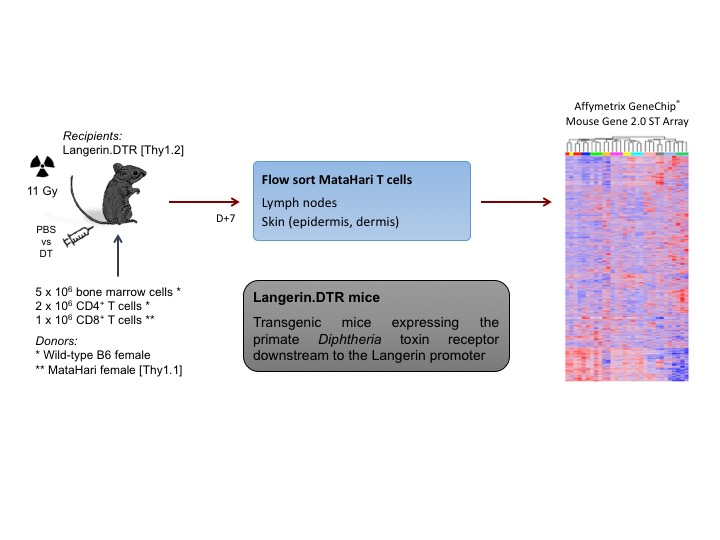
\includegraphics[width=19cm]{/cluster/project8/vyp/Winship_GVHD/vincent/GVHD/poster/figs/mataHari_DT.jpg}
        \end{minipage}
  \begin{minipage}{20cm}
    {\tiny Single minor histocompatibility antigen-mismatched BMT model. MataHari T cells, transgenic CD8 T cells that recognise a single ubiquitously-expressed male antigen (UTY peptide), were transplanted together with wild-type C57BL/6 female bone marrow and CD4 T cells into lethally irradiated C57BL/6 Langerin.DTR recipients, treated with either DT or PBS 20 days prior to BMT. Tissues were harvested at day +7 post transplant, MataHari T cells were sorted and total RNA was purified for a whole transcript expression analysis using the Affymetrix GeneChip}
        \end{minipage}



{\small	\begin{itemize} % NOT SURE THIS IS NEEDED IF MODEL DIAGRAM IS INCLUDED
\item Langerhans cells (LCs) are the predominant APCs in the skin and are radio-resistant  
\item LCs have been shown to be sufficient for GVHD progression although this theory is controversial  
\end{itemize}}

%	\begin{minipage}{0.45\textwidth}
%	\end{minipage}

%\begin{minipage}{0.45\textwidth}
% \includegraphics[width = 13cm]{/cluster/project8/vyp/Winship_GVHD/claire/results/epi_dermis_PLN/figs/matahari.pdf}  
%\end{minipage}%

\hfill

\begin{minipage}{0.45\textwidth}
       \includegraphics[width=15cm]{/cluster/project8/vyp/Winship_GVHD/claire/results/epi_dermis_PLN/figs/PCA_prettier.pdf}
      \end{minipage}
      \begin{minipage}{0.45\textwidth}
        \includegraphics[width=13cm]{/cluster/project8/vyp/Winship_GVHD/claire/results/epi_dermis_PLN/figs/epidermis_vs_epidermisDT_histogram.pdf}
      \end{minipage}

{\small
      \begin{itemize}
      \item PCA plot shows a tight cluster of samples containing data from DT treated mice although epidermis DT samples do not cluster in this manner.
      \item Two samples (one dermis and one primary lymph node (PLN)) appear as potential outliers but they do not lie so far from the rest of the data to be excluded from analysis.
  \item Histogram pf P-values comparing T-cell epidermis expression with or without Langerhans cells clearly shows a difference.
      \end{itemize}}
\end{block}

    \begin{block}{How can we use ImmGen to understand these results?}
  
  \begin{minipage}{0.45\textwidth}
    \includegraphics[width=13cm]{/cluster/project8/vyp/Winship_GVHD/claire/results/epi_dermis_PLN/figs/epidermis_vs_epidermisDT_coarse_module_association_graph.pdf}
  \end{minipage}
\hfill
\begin{minipage}{0.45\textwidth}
\includegraphics[width=13cm]{/cluster/project8/vyp/Winship_GVHD/claire/results/epi_dermis_PLN/figs/epidermis_vs_epidermisDT_fine_module_association_graph.pdf}
\end{minipage}
\hfill
%\begin{minipage}{0.45\textwidth}
{\small	  \begin{itemize}
  \item Clearly evident is a strong association to coarse module 5
  \item This module is known to be downregulated with the differentiation of immune cells
  \item genes within this module are downregulated in the epidermis DT data sets compared to epidermis alone, suggesting that the absence of LCs in this compartment may lead to abhorrent signaling following interaction with T cells. 
  \item This set of experiments provides evidence to support the interaction of effector T cells with specific tissues/compartments 
\end{itemize}}
%\end{minipage}
    \end{block}
\end{column}

%%%%%%%%%%%%%%%%%%%%%%%%%%%%%%%%%%%%%%%%
  \begin{column}{.36\linewidth}


    \begin{block}{Assessing the behaviour of Langerhans cells in different models}
  {\bf Objective:} Evaluate the differences in gene expression of Langerhans cells in the setting of an allogeneic BMT or a syngeneic BMT. 


  \begin{minipage}{20cm}
   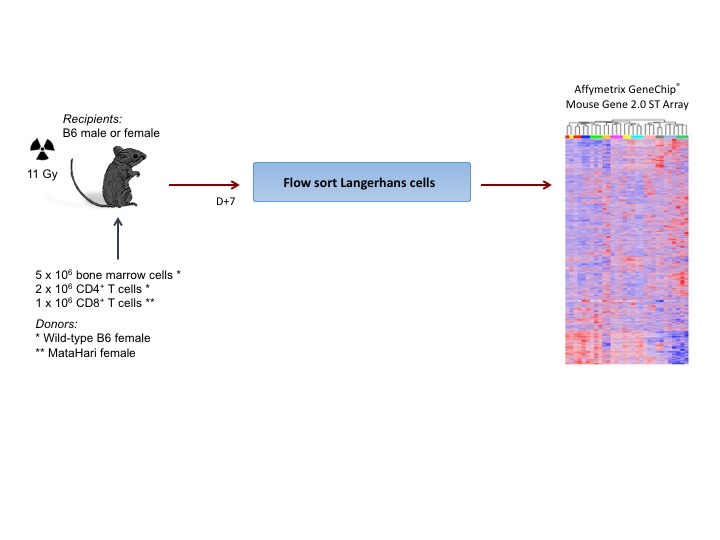
\includegraphics[width=19cm]{/cluster/project8/vyp/Winship_GVHD/vincent/GVHD/poster/figs/LangerhansCells.jpg}
        \end{minipage}
  \begin{minipage}{20cm}
    \begin{itemize}
    \item Allogeneic BMT recipients (bone marrow B6 female donor and T cells from MataHari female donor B6 male recipient)
    \item Syngeneic BMT recipients (bone marrow and T cells from B6 female donor  B6 female recipient)
    \item Untreated recipient (B6 male)
    \end{itemize}
        \end{minipage}


%	  \begin{minipage}{0.25\textwidth}
%    \includegraphics[width = 13cm]{/cluster/project8/vyp/Winship_GVHD/claire/results/epi_dermis_PLN/figs/matahari.png}
%  \end{minipage}
% {\small	\begin{itemize} - %%  NOT SURE THIS IS NEEDED IF MODEL DIAGRAM IS INCLUDED

%	\item MataHari T cells were transplanted with wild-type female bone marrow and CD4 T cells into Langerin.DTR recipients 
%	\item Mice were subsequently treated with either DT or PBS 20 days prior to BMT.
%	\item Tissues were harvested at day +7 post transplant
%	\item Uniform presentation of single male specific antigen across entire T cell population
%	\item Suggests any differences in T cell transcriptional profiles must occur in the peripheral tissues and may be the result of tissue specific T cell interactions driving GVHD
%
%	\end{itemize}}

%  \hfill


  \begin{minipage}{0.4\textwidth}
   \includegraphics[width=13cm]{/cluster/project8/vyp/Winship_GVHD/claire/results/syn_allo_bmt/figs/PCA_prettier.pdf}
      \end{minipage}
  \begin{minipage}{0.4\textwidth}
      {\small          \begin{itemize}
    \item No particularly distinct clustering of samples evident
          \end{itemize}}
  \end{minipage}
\end{block}

\begin{block}{ImmGen matching reveals hidden signals}

  
      \begin{minipage}{0.30\textwidth}
        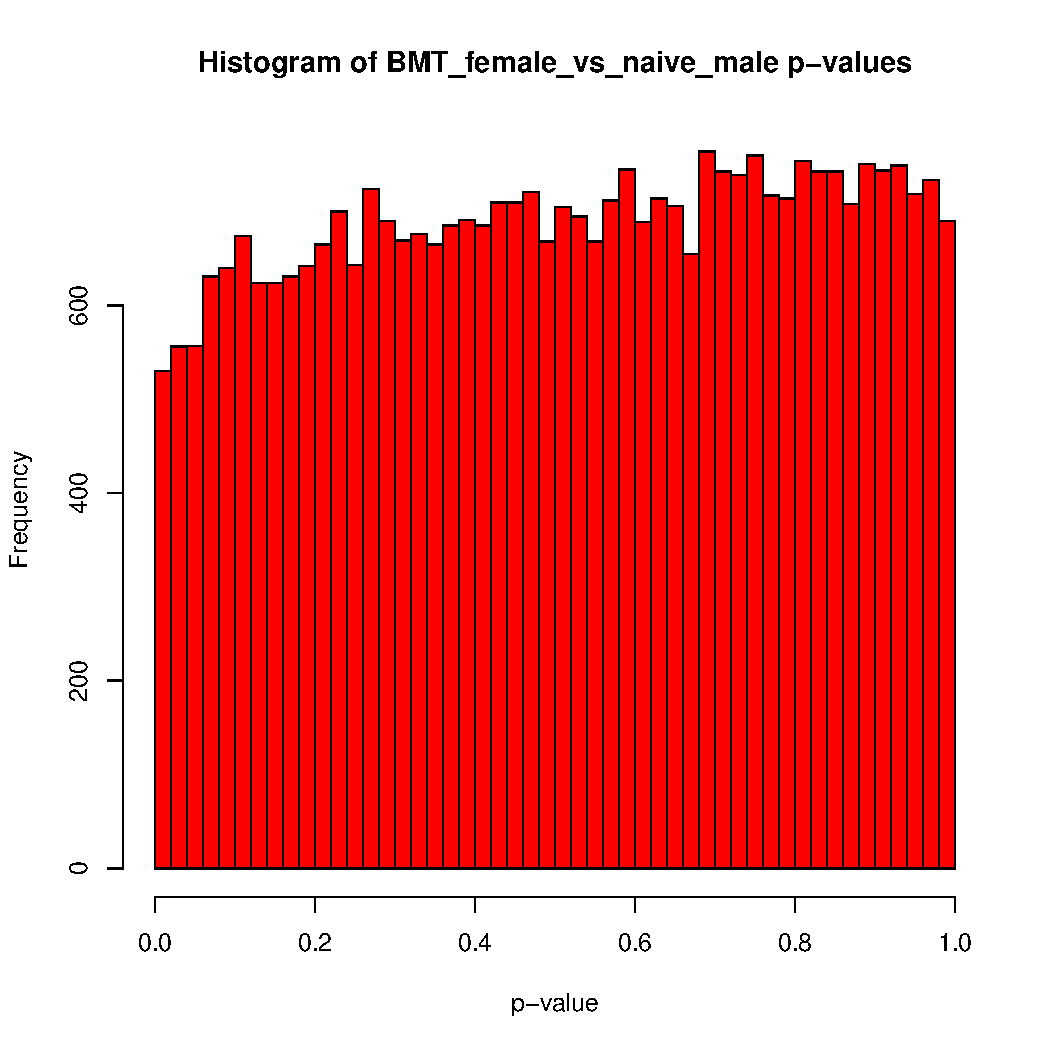
\includegraphics[width=12cm]{/cluster/project8/vyp/Winship_GVHD/claire/results/syn_allo_bmt/figs/BMT_female_vs_naive_male_histogram.pdf}
      \end{minipage}
  \hfill 
\begin{minipage}{0.30\textwidth}
        \includegraphics[width=12cm]{/cluster/project8/vyp/Winship_GVHD/claire/results/syn_allo_bmt/figs/BMT_female_vs_naive_male_coarse_module_association_graph.pdf}
      \end{minipage}
\hfill
\begin{minipage}{0.30\textwidth}
        \includegraphics[width=12cm]{/cluster/project8/vyp/Winship_GVHD/claire/results/syn_allo_bmt/figs/BMT_female_vs_naive_male_fine_module_association_graph.pdf}
      \end{minipage}
{\small \begin{itemize}
\item Increased expression of coarse module 11 genes in the BMT female mouse - this module contains many cell cycle genes
\item Majority of differentially expressed genes in coarse module 11 are also part of fine module 56 - may suggest the upregulation of one pathway/several closely related pathways 
\end{itemize}}




%\begin{minipage}{0.20\textwidth}
    %    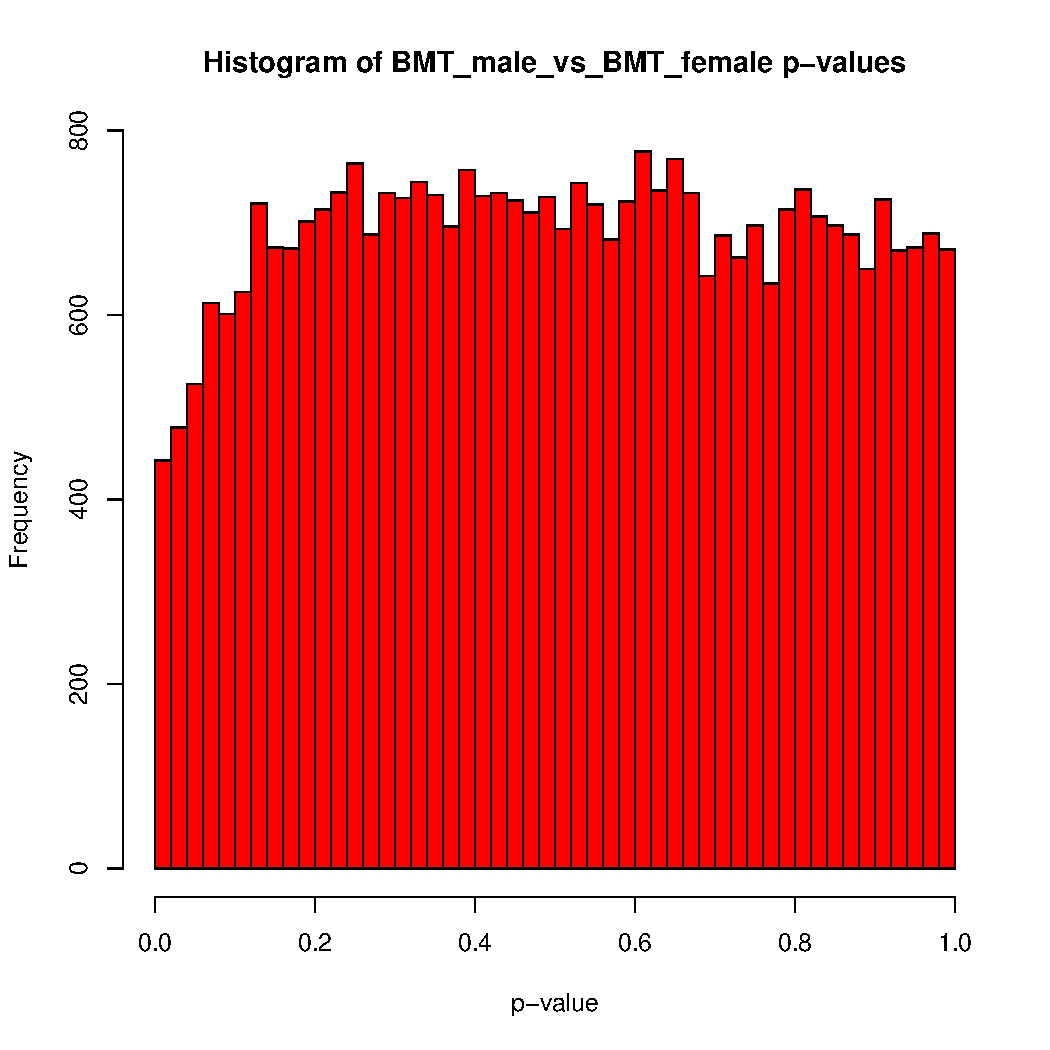
\includegraphics[width=12cm]{/cluster/project8/vyp/Winship_GVHD/claire/results/syn_allo_bmt/figs/BMT_male_vs_BMT_female_histogram.pdf}
    %  \end{minipage}
%\hfill
%\begin{minipage}{0.20\textwidth}
    %    \includegraphics[width=12cm]{/cluster/project8/vyp/Winship_GVHD/claire/results/syn_allo_bmt/figs/BMT_male_vs_BMT_female_coarse_module_association_graph.pdf}
    %    \end{minipage}
%\hfill
%\begin{minipage}{0.40\textwidth}
% {\small    \begin{itemize}
%	\item Potentially interesting association seen for Coarse module 34 
%	\item Genes within this module are associated with antigen processing and presentation and is upregulated with differentiation 
%	\item Largely downregulated in the BMT male suggesting potential disregulation of function  
%	\end{itemize}}  
%	\end{minipage}
%\hfill


\begin{minipage}{0.30\textwidth}
        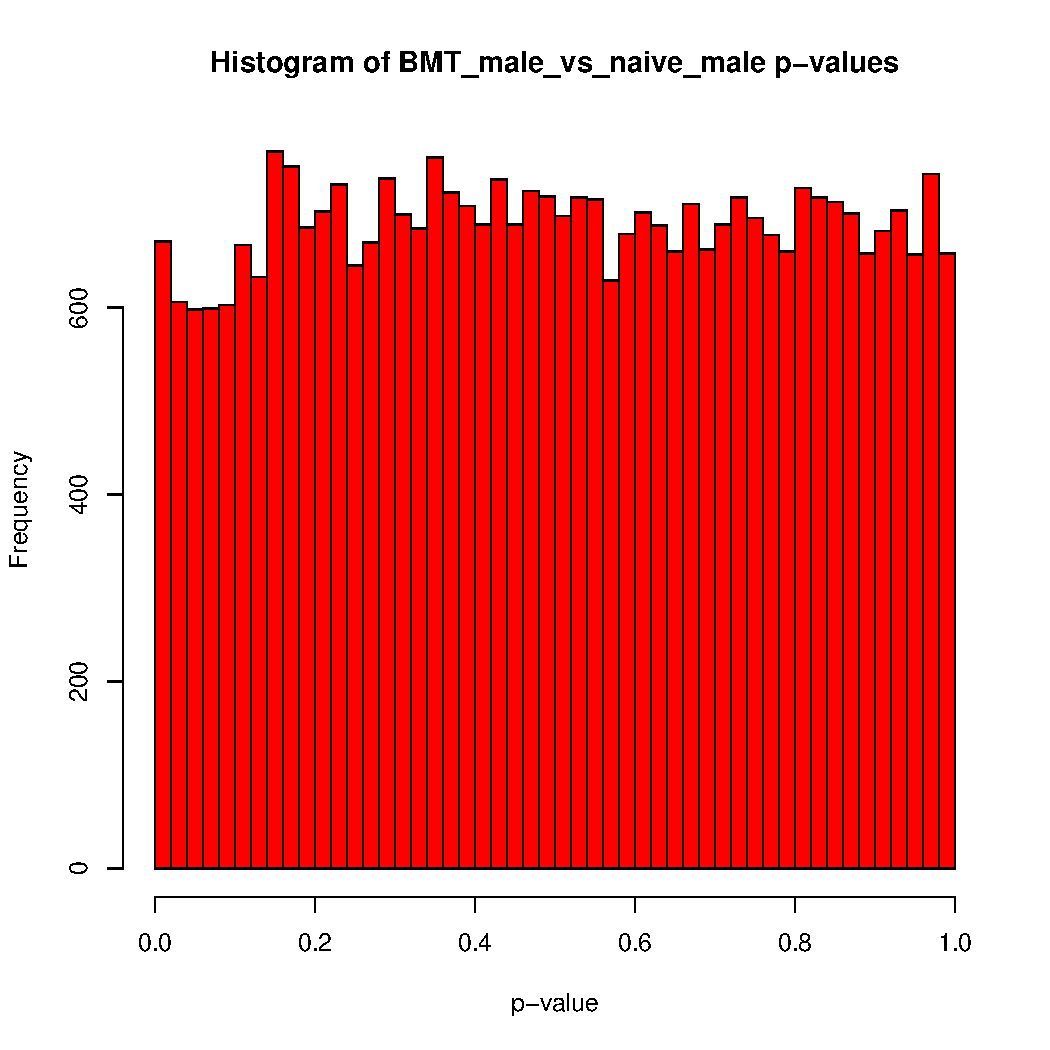
\includegraphics[width=12cm]{/cluster/project8/vyp/Winship_GVHD/claire/results/syn_allo_bmt/figs/BMT_male_vs_naive_male_histogram.pdf}
      \end{minipage}
  \hfill
      \begin{minipage}{0.30\textwidth}
        \includegraphics[width=12cm]{/cluster/project8/vyp/Winship_GVHD/claire/results/syn_allo_bmt/figs/BMT_male_vs_naive_male_coarse_module_association_graph.pdf}
      \end{minipage}
  \hfill
  \begin{minipage}{0.30\textwidth}
        \includegraphics[width=12cm]{/cluster/project8/vyp/Winship_GVHD/claire/results/syn_allo_bmt/figs/BMT_male_vs_naive_male_fine_module_association_graph.pdf}
      \end{minipage}
  \hfill
{\small \begin{itemize}
\item Histogram of BMT male vs naive male p-values appears to show a more consistent distribution with the null hypothesis
\item Again a strong association is seen for coarse module 34 suggesting slight decrease in antigen processing/presentation in the BMT male
\item Additional peak for coarse module 52 which is known to contain genes involved in the interferon response 
\item Evidence of a potentially interesting biological response despite the comparatively flat P-value histogram 
\end{itemize}}
    \end{block}




\begin{block}{Next steps}
{\small  \begin{itemize}
        \item Next step is to attempt to identify T cell expression signature within the lymph-node
    \item In vivo T cells rapidly migrate from the lymph node to peripheral tissues but this can be prevented using the drug Fingolimod (FTY720) 
     \item FTY720 is a sphingosine 1-phosphate (S1P) analogue that blocks lymphocyte egress from the lymph nodes by abrogation of T cell and sinusoid interactions.
      \item Confounding factor: how much is the T cell expression pattern a driving force of GvHD as opposed to the T cells simply behaving differently in peripheral tissues compared to the lymph node
      \item Key question: what proportion of unique peripheral tissue expression should be considered significant 
      \end{itemize}}
\end{block}
\end{column}
\end{columns}
\end{frame}
\end{document}


%%%%%%%%%%%%%%%%%%%%%%%%%%%%%%%%%%%%%%%%%%%%%%%%%%%%%%%%%%%%%%%%%%%%%%%%%%%%%%%%%%%%%%%%%%%%%%%%%%%%
%%% Local Variables: 
%%% mode: latex
%%% TeX-PDF-mode: t
%%% End:
